\documentclass[12pt,italian]{report}
\usepackage{tesi}
%\usepackage[section]{placeins}

%
%			INFORMAZIONI SULLA TESI
%			DA COMPILARE!
%

% CORSO DI LAUREA:
\def\myCDL{Corso di Laurea magistrale in\\Informatica}
% TITOLO TESI:
\def\myTitle{Il titolo\\della tesi}

% AUTORE:
\def\myName{Lorenzo D'Alessandro}
\def\myMat{Matr. Nr. 939416}

% RELATORE E CORRELATORE:
\def\myRefereeA{Relatore 1}
\def\myRefereeB{Correlatore 1}

% ANNO ACCADEMICO
\def\myYY{2020-2021}

% Il seguente comando introduce un elenco delle figure dopo l'indice (facoltativo)
%\figurespagetrue

% Il seguente comando introduce un elenco delle tabelle dopo l'indice (facoltativo)
%\tablespagetrue

%
%			PREAMBOLO
%			Inserire qui eventuali package da includere o definizioni di comandi personalizzati
%

% Package di formato
\usepackage[a4paper]{geometry}		% Formato del foglio
\usepackage[italian]{babel}			% Supporto per l'italiano
\usepackage[utf8]{inputenc}			% Supporto per UTF-8
%\usepackage[a-1b]{pdfx}			% File conforme allo standard PDF-A (obbligatorio per la consegna)

% Package per la grafica
\usepackage{graphicx}				% Funzioni avanzate per le immagini
\usepackage{hologo}					% Bibtex logo with \hologo{BibTeX}
%\usepackage{epsfig}				% Permette immagini in EPS
%\usepackage{xcolor}				% Gestione avanzata dei colori

% Package tipografici
\usepackage{amssymb,amsmath,amsthm} % Simboli matematici
\usepackage{listings}				% Scrittura di codice

% Package ipertesto
\usepackage{url}					% Visualizza e rendere interattii gli URL
\usepackage{hyperref}				% Rende interattivi i collegamenti interni


\begin{document}

% Creazione automatica del frontespizio
\frontespizio
\beforepreface

% 
%			PAGINA DI DEDICA E/O CITAZIONE
%			facoltativa, questa è l'unica cosa che dovete formattare a mano, un po' come vi pare
%

{\raggedleft \large \sl Dedica \\}
         
% 
%			PREFAZIONE (facoltativa)
%

%\prefacesection{Prefazione}
%Le prefazioni non sono molto comuni, tuttavia a volte capita che qualcuno voglia dire qualcosa che esuli dal lavoro in s\'e (come un meta-commento sull'elaborato), o voglia fornire informazioni riguardanti l'eventuale progetto entro cui la tesi si colloca (in questo caso \`e probabile che sia il relatore a scrivere questa parte).

%
%			RINGRAZIAMENTI (facoltativi)
%

\prefacesection{Ringraziamenti}
Questa sezione, facoltativa, contiene i ringraziamenti.

%
%			Creazione automatica dell'indice
%

\afterpreface

% 
%			CAPITOLO 1: Introduzione o Abstract
% 

\chapter{Introduzione}
\label{cap:introduzione}

Introduzione...

\section{I contenuti}
\label{sec:contenuti}

Spiegazione problema...


\section{Organizzazione della tesi}
\label{sec:organizzazione}

Organizzazione tesi...

% 
%			CAPITOLO 2: Stato dell'arte
% 



\chapter{Stato dell'arte}
\label{chap:stato_arte}
I recommender system sono algoritmi mirati a suggerire oggetti rilevanti agli utenti. La definizione di oggetto è generica e include ad esempio film da guardare, libri da leggere, prodotti da comprare o qualsiasi altra cosa a seconda del contesto in cui sono implementati. 
Quando gli utenti interagiscono con il sistema generano dei feedback. Questi feedback possono essere di due tipi: espliciti o impliciti. I feedback espliciti sono valori numerici che un utente assegna ad un prodotto, i feedback impliciti riflettono indirettamente le opinioni di un utente osservando la cronologia degli acquisti, i link clickati, gli elementi visualizzati, etc.
Basandosi sui feedback passati, i RS imparano un modello per prevedere quanto un utente può essere interessato a nuovi oggetti. Questi oggetti sono poi ordinati in base alla pertinenza prevista per l'utente. In ultimo, gli oggetti con il rank più alto vengono suggeriti all'utente. La relazione tra utenti e oggetti è rappresentata con una matrice $R_M$ in cui sono memorizzati i rating passati degli utenti.
La \textit{ratings matrix} è definita come: 
$$
R_M: U \times I \rightarrow R
$$
dove $U = \{u_1, \dots, u_m\}$ rappresenta l'insieme degli utenti, $I = \{i_1,\dots, i_n\}$ rappresenta l'insieme degli utenti, e $R = \{r_1, \dots, r_k\}$ rappresenta l'insieme dei possibili ratings che un utente ha espresso riguardo a degli oggetti. Un valore mancante nella ratings matrix può avere due significati: l'utente non vuole esprimere un'opinione su un oggetto specifico, oppure l'utente non conoscendo ancora l'oggetto non può averlo valutato \cite{survey-mattia}.

\vspace{5mm}
\noindent I recommender system si dividono principalmente in 3 categorie:
\begin{itemize}
	\item collaborative filtering
	\item content-based
	\item hybrid
\end{itemize}

\noindent In figura \autoref{fig:cb-cf} è schematizzato il modo diverso in cui operano i metodi collaborative filtering rispetto a quelli content-based.

\begin{figure}
  \includegraphics[width=\linewidth]{immagini/cb_cf_schema.png}
  \caption{Collaborative filtering vs Content-based}
  \label{fig:cb-cf}
\end{figure}



\section{Collaborative filtering}
Collaborative filtering (CF) è considerata la tecnica di raccomandazione più popolare e ampiamente utilizzata nei RS. Il presupposto alla base di CF è che le persone con preferenze simili valuteranno gli stessi oggetti con ratings simili. CF quindi sfrutta le informazioni sul comportamento passato o le opinioni di una comunità di utenti esistente per prevedere quali elementi potranno piacere o saranno interessanti per l'utente corrente del sistema \cite{recsys-intro}. Gli approcci CF puri non sfruttano né richiedono alcuna conoscenza degli oggetti stessi ma solo dei feedback degli utenti.

La classe di algoritmi più famosa è quella di Matrix Factorization, ma recentemente sono stati sviluppati diversi approcci basati sul deep learning \cite{deep-learning-survey}.

\subsection{Vantaggi e svantaggi} \label{ssec:pros-cons-cf}
\textbf{Vantaggi:}
\begin{itemize}

 \item \textit{Nessuna conoscenza del dominio necessaria:} il modello può funzionare in domini in cui non c'è molto contenuto associato agli oggetti e in cui il contenuto è difficile da analizzare per un sistema informatico (come opinioni e ideali) \cite{recsys-principle-methods-evaluation}.
 
 \item \textit{Serendipity:} il modello ha la capacità di fornire consigli fortuiti, il che significa che può consigliare elementi pertinenti per l'utente anche senza che il contenuto si trovi nel profilo dell'utente permettendo all'utente di scoprire nuovi interessi \cite{recsys-principle-methods-evaluation} \cite{cf-advantages-google}.
\end{itemize}

\noindent \textbf{Svantaggi:}
\begin{itemize}
 \item \textit{Problema del cold-start:} Si riferisce alla situazione in cui il sistema di raccomandazione non ha abbastanza informazioni su un utente od un oggetto per poter fare previsioni rilevanti. Un nuovo oggetto inserito nel RS di solito non ha voti, ed è quindi improbabile che venga raccomandato. Un oggetto non consigliato passa inosservato a gran parte della community. Il problema è presente anche per i nuovi utenti: gli utenti che hanno espresso nessuna o poche valutazioni non ricevono raccomandazioni affidabili \cite{cold-start}.   
 
 \item  \textit{Problema di data sparsity:} questo è il problema che si verifica a causa della mancanza di informazioni sufficienti, cioè quando solo pochi rispetto al numero totale di oggetti disponibili in un database sono valutati dagli utenti. Ciò porta ad una rating matrix sparsa, e raccomandazioni poco efficaci \cite{recsys-principle-methods-evaluation}.
 
 \item \textit{Scalabilità:} Questo è un altro problema associato agli algoritmi di raccomandazione perchè il tempo di computazione cresce linearmente con il numero di utenti e oggetti. Un sistema di raccomandazione efficiente con un dataset limitato potrebbe non esserlo quando il volume è incrementato \cite{recsys-principle-methods-evaluation}.
\end{itemize}

\subsection{Matrix factorization}
Gli algoritmi basati su matrix factorization(MF) caratterizzano sia utenti che oggetti mediante dei vettori di fattori estratti dai pattern sui ratings. Una corrispondenza alta tra i fattori di un utente e un oggetto porta ad una raccomandazione. Questi metodi sono diventati popolari negli ultimi anni perchè combinano scalabilità e accuratezza.

Più formalmente, i modelli basati su matrix factorization mappano utenti e oggetti in uno spazio di fattori latenti di dimensionalità $f$, tale che le interazioni tra utenti e oggetti sono modellate come prodotti in quello spazio. Di conseguenza, ogni oggetto $i$ è associato con un vettore $q_i \in \mathbb{R}^f$, e ogni utente $u$ con un vettore $p_u \in \mathbb{R}^f$. Per un dato oggetto $i$, gli elementi di $q_i$ indicano la misura in cui l'oggetto possiede quei fattori, positivi o negativi. Per un dato utente $u$, gli elementi di $p_u$ indicato l'entità dell'interesse che l'utente ha per gli oggetti che hanno un valore alto sui fattori corrispondenti, positivi o negativi. Il prodotto scalare $q_i^Tp_u$ indica l'interesse dell'utente $u$ per le caratteristiche dell'oggetto $i$ \cite{matrix-factorization}. Quindi il rating $r_{ui}$ può essere approssimato come

\begin{equation} \label{eq:dot_product}
r_{ui} = q_i^Tp_u
\end{equation}

Il problema principale è calcolare il mapping di ogni oggetto e utente su dei vettori $q_i, p_u \in \mathbb{R}^f$. Una volta che il recommender system ha completato il mapping, può facilmente stimare il rating che un utente darà a qualsiasi oggetto utilizzando l'equazione \ref{eq:dot_product}. 

In \autoref{fig:matrix_factorization} è mostrato come la matrice dei ratings $A \in \mathbb{R}^{m \times n}$, con $m$ numero di utenti e $n$ numero di oggetti, viene decomposta in due matrici di dimensionalità minore:

\begin{itemize}
	\item Una matrice di embedding per gli utenti $P \in \mathbb{R}^{m \times f}$, in cui la riga $i$ è l'embedding dell'utente $i$
	\item Una matrice di embedding per gli oggetti $Q \in \mathbb{R}^{n \times f}$, in cui la colonna $j$ è l'embedding dell'utente $j$
\end{itemize}

Gli embedding di $P$ e $Q$ sono imparati in modo tale che il prodotto $PQ^T$ sia una buona approssimazione della matrice dei ratings $A$

\begin{figure}
  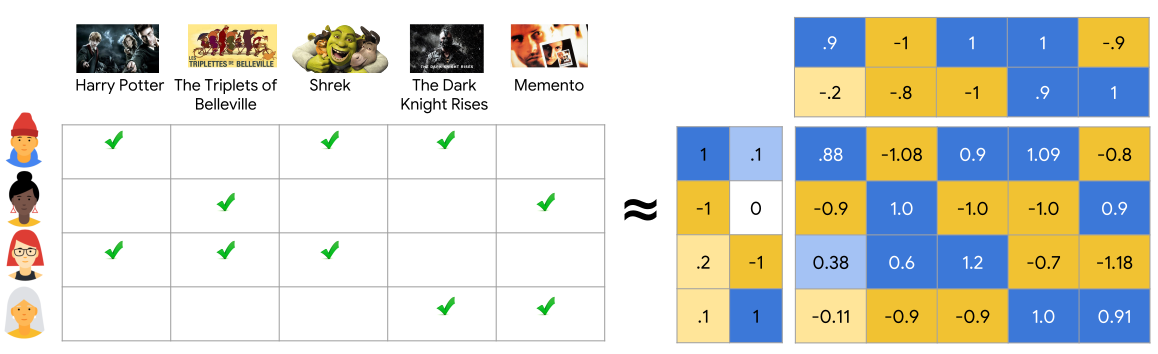
\includegraphics[width=\linewidth]{immagini/matrix_factorization.pdf}
  \caption{Approssimazione matrice dei ratings con matrix factorization}
  \label{fig:matrix_factorization}
\end{figure}

\section{Content-based}
Nei recommender system content-based (CB), gli attributi descrittivi degli oggetti sono usati per produrre raccomandazioni. Il termine "content" indica queste descrizioni. Nei metodi content-based, i ratings degli utenti sono combinati con le informazioni disponibili per gli oggetti, per poi essere usati come training data per creare un modello di classificazione o regressione specifico per l'utente. Questo modello specifico dell'utente viene utilizzato per prevedere se alla persona corrispondente piacerà un articolo per il quale la sua valutazione è ancora sconosciuta \cite{recsys-book}.

Mentre nei CF la similarità tra due oggetti (o due utenti) è calcolato come la correlazione o la similarità tra i ratings forniti dagli altri utenti, i recommender system content-based sono progettati per consigliare oggetti simili a quelli che l'utente ha preferito in passato. Non considerando gli altri utenti, la lista di raccomandazioni può essere generata anche se c'è un solo utente.

\subsection{Vantaggi e svantaggi}
\textbf{Vantaggi:}
\begin{itemize}
 \item \textit{Consigliare nuovi oggetti:} Questi modelli hanno la capacità di consigliare nuovi oggetti anche se non ci sono valutazioni fornite dagli utenti a differenza dei modelli collaborative filtering \cite{recsys-principle-methods-evaluation}.

 \item ???
\end{itemize}

\noindent \textbf{Svantaggi:}
\begin{itemize}
 \item \textit{Features degli oggetti:} la precisione del modello dipende dall'insieme delle features che descrivono gli oggetti. Identificare le features più rilevanti non è semplice e dipende molto dall'applicazione specifica \cite{survey-mattia}.
 
 \item \textit{Content overspecialization:} Dato che i metodi CB si affidano solo alle caratteristiche degli oggetti già valutati dall'utente corrente, egli riceverà solo raccomandazioni simili ad altri oggetti già definiti nel suo profilo \cite{recsys-principle-methods-evaluation}.
 
 \item \textit{Dimensione training set:} In modo da consentire a un RS content-based di imparare le preferenze di un utente, egli dovrà valutare un numero sufficiente di oggetti. In caso contrario, il RS non avrà sufficienti informazioni per imparare un modello accurato e fallirà nel raccomandare oggetti a utenti con pochi o nessun ratings.
\end{itemize}

\section{Hybrid}
I modelli ibridi combinano tipi diversi di sistemi di raccomandazione per formare dei modelli in grado di superare le debolezze dei modelli singoli. In \cite{recsys-book} sono descritti tre modi per creare recommender system ibridi:

\begin{enumerate}
 \item \textit{Ensemble design:} Con questo metodo i risultati degli algoritmi base sono combinati in un output singolo più robusto. Il principio fondamentale è molto simile ai metodi di ensemble usati in molte applicazioni di data mining come clustering, classificazione e analisi degli outlier. 
Gli ensemble design possono essere formalizzati nel modo seguente. Sia $R^k$ una matrice $m \times n$ contenente le predizioni di $m$ utenti per $n$ oggetti dell'algoritmo k-esimo, con $k \in \{1, \dots ,q\}$. Pertanto, un totale di $q$ algoritmi diversi sono usati per ottenere queste predizioni. L'elemento $(u,j)$-esimo di $R^k$ contiene il rating predetto per l'utente $u$ sull'oggetto $j$ dall'algoritmo $k$-esimo. Gli elementi della matrice originale $R$ sono replicati in ogni $R^k$, e solo gli elementi non presenti in $R$ variano nei differenti $R^k$ a causa dei diversi risultati degli algoritmi. Il risultato finale è ottenuto combinando le predizioni $R^1, \dots, R^q$ in un singolo output. La combinazione può essere fatta in vari modi, ad esempio calcolando la media pesata delle varie predizioni. Le caratteristiche comuni di questi algoritmi sono usare sistemi di raccomandazione già esistenti e produrre uno score/ranking unico.
 \item \textit{Monolithic design:} In questo caso, viene creato un algoritmo di raccomandazione integrato utilizzando vari tipi di dati. A volte non esiste una chiara distinzione tra le varie parti (es. content-based e collaborative filtering) dell'algoritmo. In altri casi, potrebbe essere necessario modificare gli algoritmi algoritmi di raccomandazione esistenti per essere usati all'interno dell'approccio generale, anche quando c'è una chiara distinzione tra gli algoritmi utilizzati.  Pertanto, questo approccio tende a integrare più strettamente le varie fonti di dati e non è possibile visualizzare facilmente i singoli componenti come black-boxes separate.
 \item \textit{Mixed systems:}  Come per gli ensembles, questi sistemi usano diversi algoritmi di raccomandazione come black-boxes, ma gli oggetti raccomandati dai vari sistemi sono presentati insieme senza essere combinati.
\end{enumerate} 


% 
%			CAPITOLO 3: Lavoro svolto
% 

\chapter{Classificatore}
\label{chap:classificatore}



% 
%			CAPITOLO 4: Datasets
% 

\chapter{Datasets}
\label{chap:datasets}


% 
%			CAPITOLO 5: Risultati
% 

\chapter{Risultati}
\label{chap:risultati}


% 
%			CAPITOLO 6: Conclusioni e sviluppi futuri
% 

\chapter{Conclusioni}
\label{cap6}

\section{Conclusioni}

Conclusioni...

\section{Sviluppi futuri}

Sviluppi futuri...



%
%			BIBLIOGRAFIA
%

\bibliographystyle{unsrt}
\bibliography{bibliografia}
\addcontentsline{toc}{chapter}{Bibliografia}


\end{document}


 
